% !TEX TS-program = xelatex
% !TEX encoding = UTF-8 Unicode
\documentclass[AutoFakeBold]{MyFormat}

\usepackage{listings, cite, ulem}

\lstset{
 columns=fixed,       
 numbers=left,                                        % 在左侧显示行号
 numberstyle=\tiny\color{gray},                       % 设定行号格式
 frame=none,                                          % 不显示背景边框
 backgroundcolor=\color[RGB]{245,245,244},            % 设定背景颜色
 keywordstyle=\color[RGB]{40,40,255},                 % 设定关键字颜色
 numberstyle=\footnotesize\color{darkgray},           
 commentstyle=\it\color[RGB]{0,96,96},                % 设置代码注释的格式
 stringstyle=\rmfamily\slshape\color[RGB]{128,0,0},   % 设置字符串格式
 showstringspaces=false,                              % 不显示字符串中的空格
 language=c++,                                        % 设置语言
}

\begin{document}
%=====%
%
%封皮页填写内容
%
%=====%

% 标题样式 使用 \title{{}}; 使用时必须保证至少两个外侧括号
%  如: 短标题 \title{{第一行}},  
% 	      长标题 \title{{第一行}{第二行}}
%             超长标题\tiitle{{第一行}{...}{第N行}}

\title{{个人思考}}
\entitle{{关于未来研究的思考}}
\author{Sillin Ini\\Pinyi Huang}
\maketitle
\thispagestyle{empty}
\newpage

%生成目录
\tableofcontents
\thispagestyle{empty}
\newpage

%文章主体
\mainmatter




% =======正文从第一章开始
\setcounter{chapter}{0}

\chapter{个人思考内容}
\section{个人的奇思妙想}
\subsection{关于动作单元AU}
\par AU是一个在FACS(\textit{Facial Action Coding System},面部行为编码系统)
提出的先验概念,在所有
使用到AUs的方法中,均默认AU是正确并可行的,如使用AU作为GCN中的邻接矩阵进行归一化。
是否存在一种可能,\underline{可以采用不同的特征作为邻接矩阵或提取特征的单位},
由此可以得到更好的空间特征提取的效果?
\par 理由:
\begin{enumerate}
    \item 往大了说:AU可以有很多种不同的划分方式,例如可以划分为11、
    16或36个ROI人脸兴趣区域\upcite{zhang2021short},是否有可能采用这些划分方式,
    可以达到更好的特征提取或分类效果?
    \item 往小了说:是否将一整个AU区域进行特征提取,会带有一定程度的图像噪声,或将更多不相关
    的特征同时提取进来?
\end{enumerate}
\par 缺点:
\begin{enumerate}
    \item 若采用ROI的方式,最后还是只能使用光流进行特征提取,最后又回到原点;
    \item 若要将AUs进一步细分,则可能需要人工对视频样本进行标定,提高成本;
\end{enumerate}

\subsection{关于样本集}
\par 这里存在着一个矛盾点:越复杂的神经网络就需要越庞大的训练集和样本数量,由此才能具备更好的分类
效果和防止严重的过拟合,而微表情数据库一直很稀缺;若是采用结构稍简单的神经网络,就无法达到更好的
分类性能。
\par 由此想到了,是否可以通过预处理,对视频样本的数量进行一定程度的增广,由此扩大样本数量
\upcite{wang2020micro}(即老师于2020年发表的论文),便可以更好地对神经网络进行训练。

\subsection{关于神经网络模型的想法}
\par 根据论文\upcite{zhang2021short}中的描述,其认为Encoder of Transformer具有很高的研究价值,
并提出希望他们的研究能够有助于推进未来对于Transformer的深入研究。
\par 论文原话:\textit{\uline{These findings strongly
motivate further research on the use of transformer based
architectures rather than convolutional neural networks in
micro-expression analysis, and we hope that our theoretical
contributions will help direct such future efforts}}
\par \textit{这些发现强烈地激发了对在微表达分析中使用基于变压器的架构而不是卷积神经网络的进一步研究,
我们希望我们的理论贡献将有助于指导这些未来的努力。}
\par 这篇论文中完全摒弃了CNN而使用了Encoder of Transformer来进行短期和长期空间关系的提取,
其创新点在于:虽然同为特征提取,但两者有一个很重要的区别。
\par 对于CNN来说:\textit{\uline{CNN仅在固定窗口大小内提取短期特征,
无法提取全局的长期特征。}}
\par 对于Encoder来说:\textit{\uline{而Encoder的Self-Attention可以很好地解决这个问题。}}
\begin{figure}[!h]
    \centering
    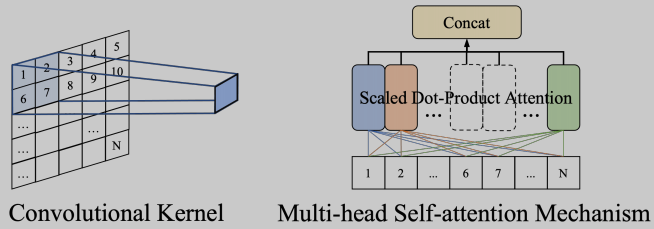
\includegraphics[width=0.9\linewidth]{figures/MyReflections/1.png}
    \caption{两种不同的空间特征提取方法的对比}
\end{figure}
\par 而其完整的神经网络SLSTT模型结构图如下:
\begin{figure}[!h]
    \centering
    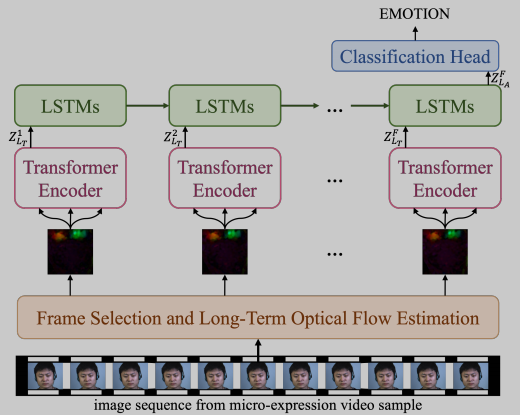
\includegraphics[width=0.6\linewidth]{figures/MyReflections/2.png}
    \caption{SLSTT模型总体结构}
\end{figure}
\par 那么是否存在一种可能,我们可以对Transformer的结构进行更进一步的研究,从而提出一些更好的基于
Encoder of Transformer的模型进行MER任务?关于论文\upcite{zhang2021short}的大致总结如第二章所示。



\subsection{关于梯度下降方法的想法}
\par 由于微表情数据的稀缺,即使是最大的数据库,其包含的样本也很少。由此必须采用一些方法,来防止
严重的过拟合现象发生,如:随着神经网络参数逐渐接近最佳时,学习率需要适当降低。
\par 受\upcite{zhang2021short}启发,可以采用\textit{cosine annealing}\upcite{faceplusplus}
方法(\underline{暂时还没具体去了解是什么})。
\par 但是在Pytorch的优化器(\textit{torch.optim})中,有一类优化器SGD(
\textit{stochastic Gradient Decent})随机梯度下降可以采用冲量进行梯度下降。
这样的梯度下降算法,在每一步时都会考虑到上一步的更新量,由此达到更好的收敛效果。是否
\textit{cosine annealing}是比SGD等优化器更好的方法?


\subsection{关于人种问题}
\par 有一个很细节的问题:\underline{当考虑人种问题时,所有方法的准确率都出现了明显的下滑}。所有
MER方法在CASME II上的识别率都显然高于其他数据库\upcite{zhang2021short},而CASME II
内只有中国人的样本。\
\par 是否有可能改进这一现象,由此能够写一篇论文?
\par 根据论文\upcite{zhang2021short}的描述,
这一问题:\textit{\uline{The performance of all methods 
on CASME II is consistently higher than when applied on other data sets, 
which suggests that the challenge of MER is increased with ethnic diversity of 
participants – this should be born in mind in future research and any comparative analysis.}}
\par CASME II中所有方法的表现始终高于应用于其他数据集的方法,
这表明MER的挑战随着受试者的种族多样性而增加——这应该在未来的研究和任何比较分析中牢记。



\chapter{关于已读论文}
\section{\textit{Short and Long Range Relation
Based Spatio-Temporal Transformer for
Micro Expression Recognition(2021.12)}\cite{zhang2021short}}
\par 个人的一些总结:

\begin{enumerate}
    \item 将视频中每一帧与微表情起始帧计算光流场,而非任意两连续帧。\\
    计算相邻帧之间的光流场时,在前半部分有相似的光流,后半部分则强度相似,方向相反。\\
    而用这里提出的方法,发现光流场总是沿同样的方向,只是前半部分的强度逐渐递增,
    后半部分的强度逐渐递减。这导致了与每个微表情相关的更稳定和可区别的特征。
    \item \textbf{\Large \underline{首个}}完全摒弃CNN进行特征提取的MER神经网络模型。
    其认为,CNN只能在固定窗口大小中进行短期空间特则提取,由此无法学习到同样十分重要的长期空间特征。
    而Encoder of Transformer中使用到的Multi-head Self-attention Mechanism(MSM)自注意力
    机制,可以很好的学习到短期和长期空间特征,由此其完全摒弃了CNN的使用。
    \item 时间聚合:使用了LSTM Aggregator进行聚合,并与Mean Aggregator进行了对比。聚合函数确保了Transformer模型可以被训练并应用于每一帧的空间特征集,然后处理每个样本中各帧之间的时间关系。
\end{enumerate}
\par 其具体细节的总结和个人理解见2022.07.31.pdf

\normalem
\bibliographystyle{ieeetr}
\bibliography{bib/Literatures}
\end{document}